During \textit{RNA-seq} data analysis, it is almost mandatory to explore the data during each step of the analysis, in order to understand which is the best method to apply for, at each analysis step and to be more confident with produced results. 

At this scope, we equipped \gls{tic} of several useful graphics and plots to be used at each analysis step.

Each of them, except when otherwise declared, with aim of \textit{plotly} library, enables to convert the plot in an interactive \textit{HTML} plot, useful to inspect additional attributes with the mouse pointer.

\subsubsection{Exploration Plots on Counts}
As already mentioned (section \ref{sec:ticorsernormalization}), the normalization phase critically affects the final results in terms of \glspl{deg} detected.
That's why it is a good norm to always understand how the applied transformations are influencing the counts. 
To address this need we implemented two plots, the \textit{Boxplot} and the \gls{pca}.

The \textit{boxplot} is a graphical representation of the distribution of the samples. 
Our \textit{boxplot} is organized in group colours accordingly to the time-point each sample belongs to (figure \ref{fig:ticorserboxplot}).

Each box is divided in two main parts, with an outgoing segment from each side. 
The horizontal upper and lower lines of the box represent the first and third quartile, while the middle horizontal rule represents the median.
The upper and lower part of the segments represent the minimum and maximum values of the sample distribution.

\begin{figure}[H]
\centering
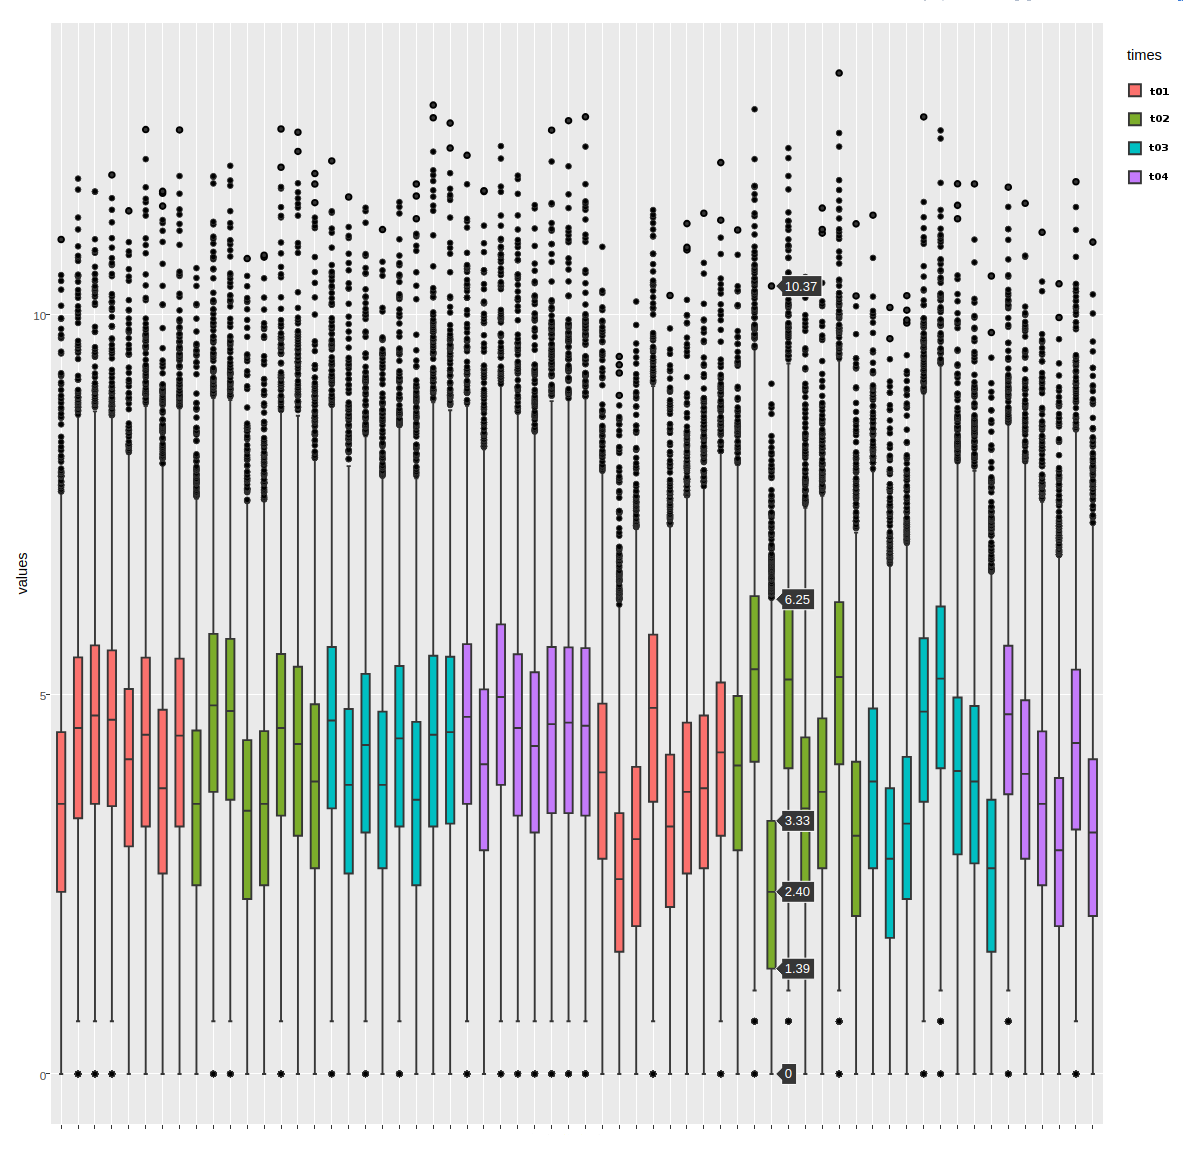
\includegraphics[width=10cm, keepaspectratio]{img/ticorser/boxplot_example.png}
\caption[ticorser boxplot]{An example of interactive boxplot made with \gls{tic} package. Each boxplot represents a specific sample, while each colour represents a specific time point. When passing the mouse over a boxplot it shows additional information about its quartiles.}
\label{fig:ticorserboxplot}

\end{figure}

Our \lstinline!plotBoxplotPlotly! function is based on the design matrix, describing the data counts, which gives the possibility to select the column to use for coloring the samples thanks to the \lstinline!colorColname! parameter. 

Due to the very high dimensionality of \textit{RNA-seq} data, it is widely considered common sense to apply \gls{pca} dimensionality reduction technique to visualize the data, limiting their representation to 2 or 3 dimensions.
There are several packages allowing to apply a \gls{pca} transformation, but we choose to implement it in the \lstinline!PlotPCAPlotlyFunction! function, by using the \lstinline!prcomp! from the \textit{stats} package.


\begin{figure}[H]
\centering
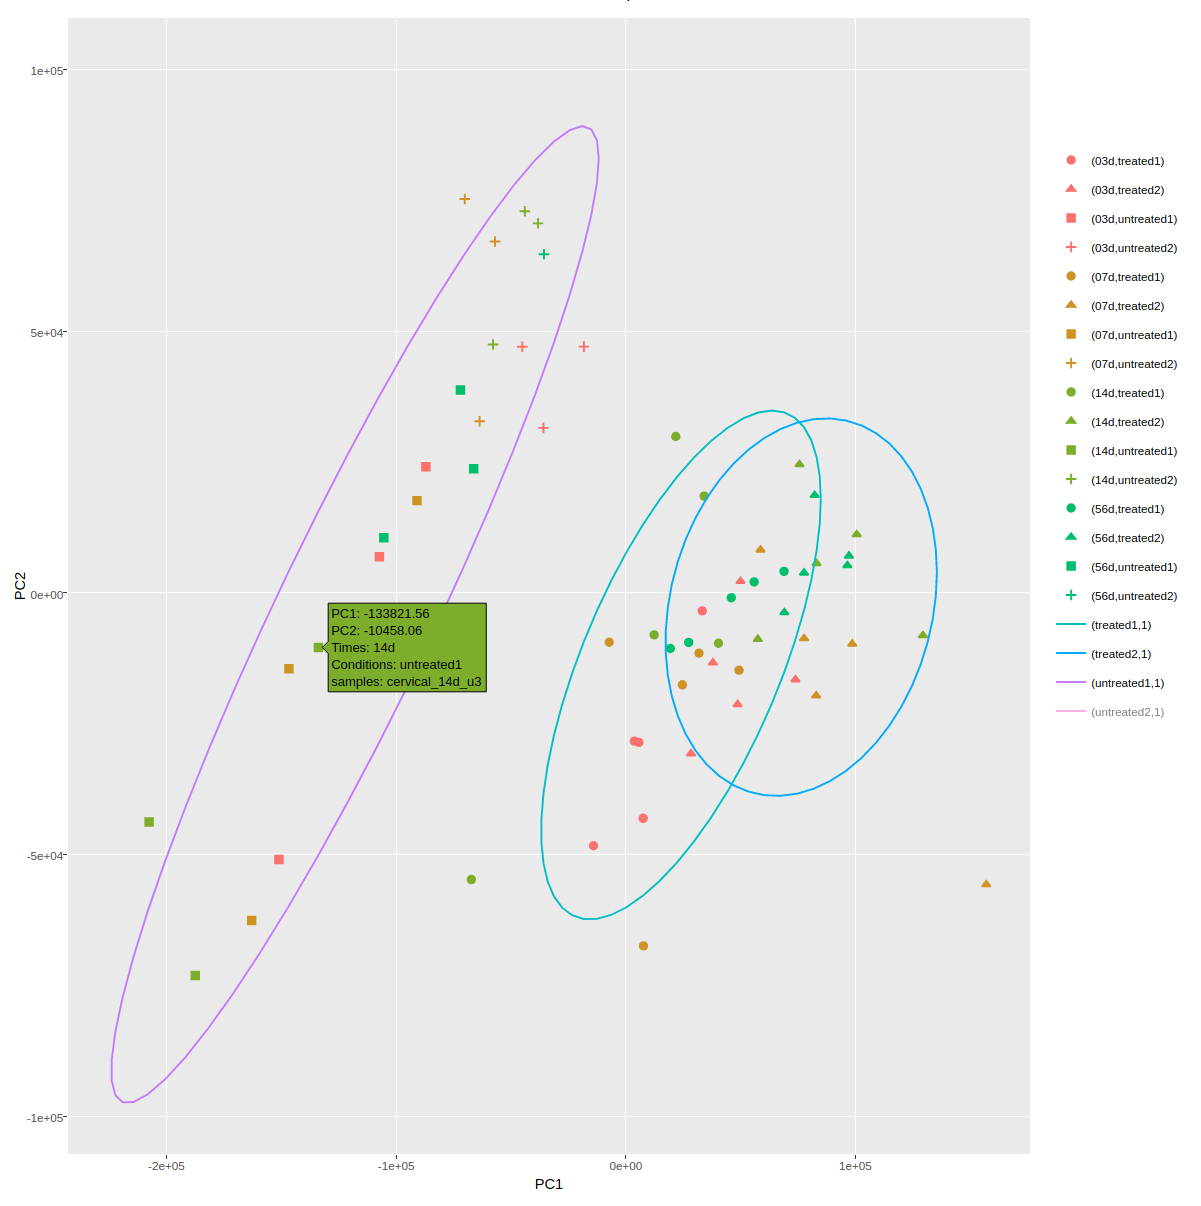
\includegraphics[width=\textwidth, keepaspectratio]{img/ticorser/pca_example.png}
\caption[ticorser pca]{An example of interactive \gls{pca} made with \gls{tic} package. Each dot represents a specific sample, while each colour represents a time point, each symbol represents a biological condition group. When passing the mouse over a dot it shows additional information about the selected sample, while from the legend it's possible to show/hide groups or ellipses.}
\label{fig:ticorserpca}

\end{figure}


The user just needs to give the \lstinline!counts.data.frame! and the \lstinline!design.data.frame! by specifying the column name where to find the samples groups.
In such a way, the function will compute and plot the \gls{pca}, coloring the samples according to the groups identified by the chosen column.
It is also possible to specify the \glspl{pc} to plot with \lstinline!xPCA! and \lstinline!yPCA!, where x and y indicate respectively the x-axis and y-axis.
Moreover, by setting the \lstinline!ellipse.flag! argument to \lstinline!TRUE!  the function will show the ellipses surrounding each sample group, each one describing the variance of the groups.

\begin{figure}[H]
\centering
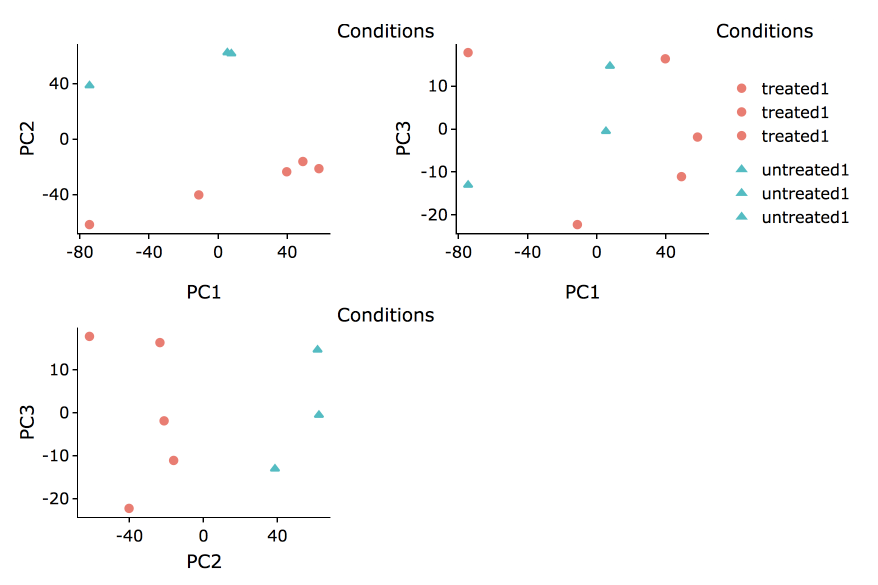
\includegraphics[width=\textwidth, keepaspectratio]{img/ticorser/pcas.png}
\caption[ticorser pca]{An example of interactive matrix \gls{pca} made with \gls{tic} package. Each plot puts in relation two different Principal Components. While each dot represents a specific sample, while each colour represents a time point, each symbol represents a biological condition group. When passing the mouse over a dot it shows additional information about the selected sample, while from the legend it's possible to show/hide groups or ellipses.}
\label{fig:ticorserpcas}
\end{figure}

In order to plot more than one \glspl{pc}, \gls{tic} allows to plot more than one comparison between them at the same time (figure \ref{fig:ticorserpcas}).
By using the \lstinline!plotPCAMatrixPlotly! function it's possible to compare more than two \glspl{pc} at the same time, simply by using the \lstinline!pca.list! argument.


\subsubsection{DE Results Plots}
In order to inspect the results produced by so many different \textit{DE} methods, we implemented two kind of plots, the \textit{VolcanoPlot} and the \textit{MAPlot}.

Both our implemented methods take as input a \textit{DE} results data frame, automatically recognizing which method produced it, lightening, in such a way, the user load during the analysis.
Moreover, it gives the possibility to add a list of positive control genes, in order to annotate them on the volcano plot with a third color (figure \ref{fig:ticorservolcano}).

The volcano plot shows the relation of $log_2(FC)$ with $log_{10}(p-value)$ of each gene, in order to highlight the significant changes inside the data experiment.

\begin{figure}[H]
\centering
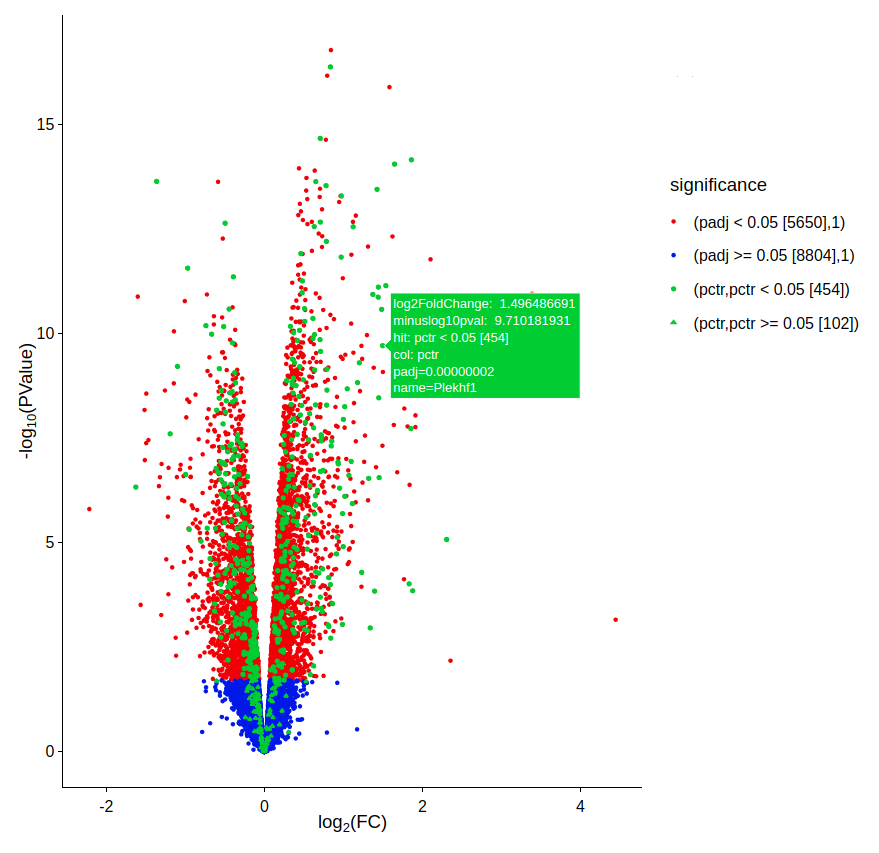
\includegraphics[width=10cm, keepaspectratio]{img/ticorser/volcano_example.png}
\caption[ticorser volcano]{An example of interactive volcano plot made with \gls{tic} package. Each dot represents a gene, while blue and red colours highlights the significance of the genes. In green there are those genes coming from the positive control list. When passing the mouse over a dot it shows additional information about the selected gene.}
\label{fig:ticorservolcano}
\end{figure}

The MA-Plot shows the relation between two quantities useful to understand the differences between the measurements in two conditions.
On the x-axis there is represented the $log_2(FC)$, where \textit{FC} is the fold change computed as the ratio of the treatment on the reference.
It is not mandatory to have a DE results dataframe to plot an MA-plot, but it's pretty useful to have it in order to highlight the distribution of the significant genes (figure \ref{fig:ticorsermaplot}).
 
\begin{figure}[H]
\centering
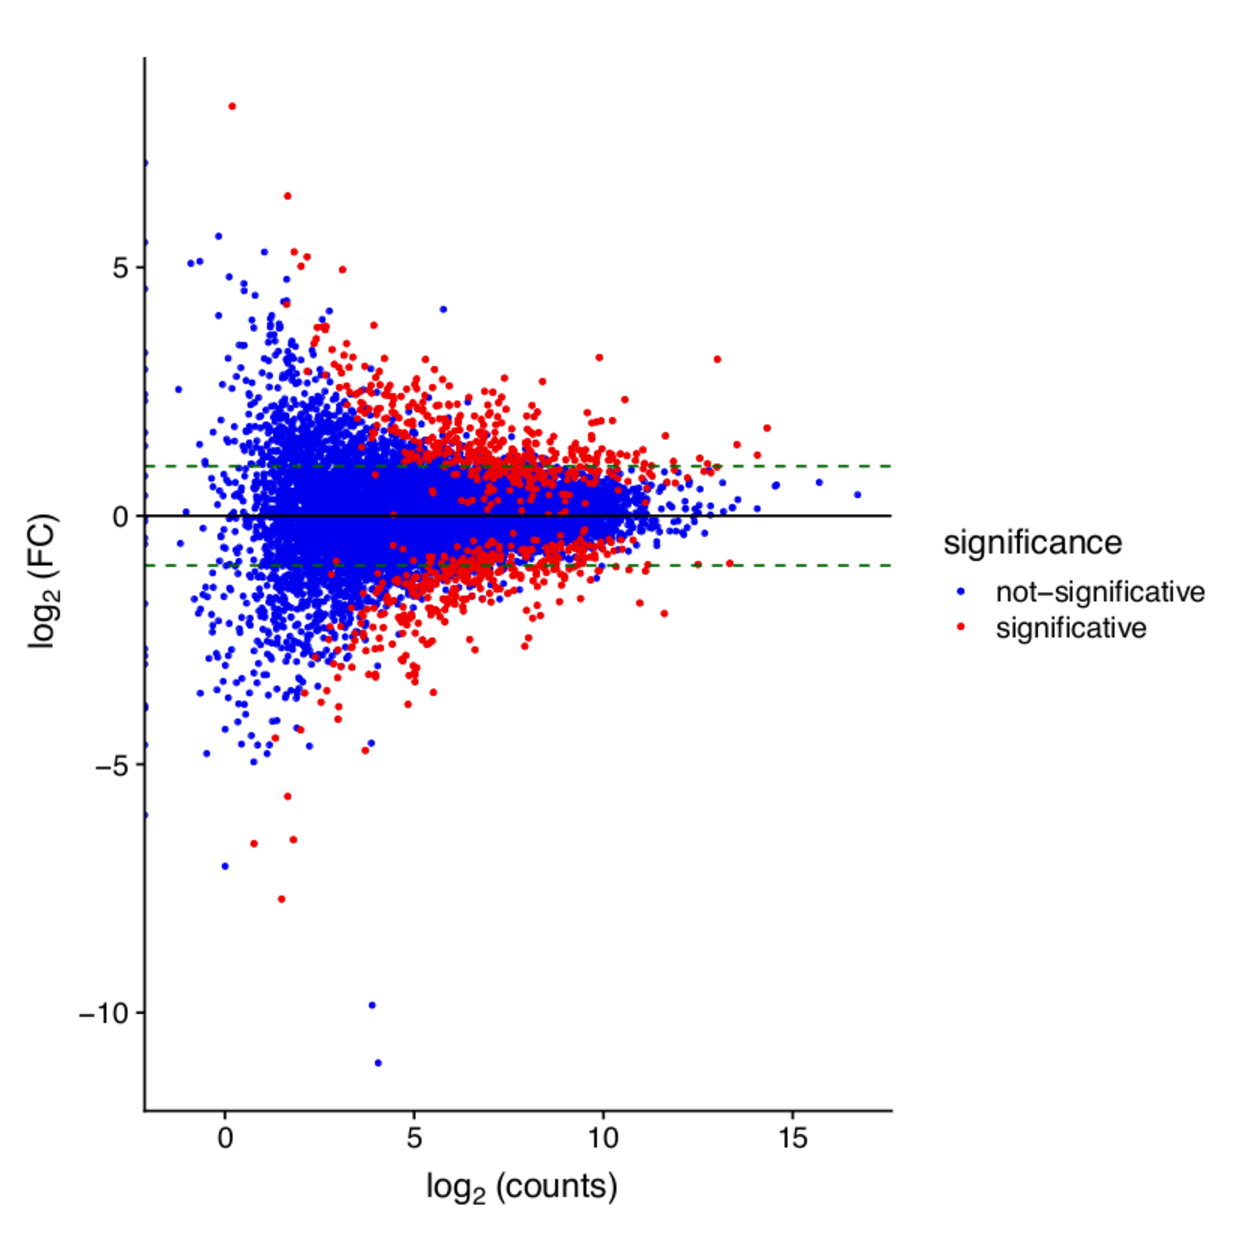
\includegraphics[width=10cm,keepaspectratio]{img/ticorser/maplot.pdf}
\caption[ticorser MAplot]{An example of interactive MA-plot made with \gls{tic} package. Each dot represents a gene, while blue and red colours highlights the significance of the genes. When passing the mouse over a dot it shows additional information about the selected gene.}
\label{fig:ticorsermaplot}
\end{figure}


\subsubsection{Gene Profiles plot}
When working with time course data experiment, it is really useful to understand the trend of one or more genes across all the time points and of one condition in relation to the other.

In order to highlight the gene expression of a gene across multiple time points and different conditions, we implemented the \lstinline!plotGeneProfile! function, which takes as input a count matrix, its linked design matrix and a gene name (figure \ref{fig:ticorsertrends}).

\begin{figure}[H]
\centering
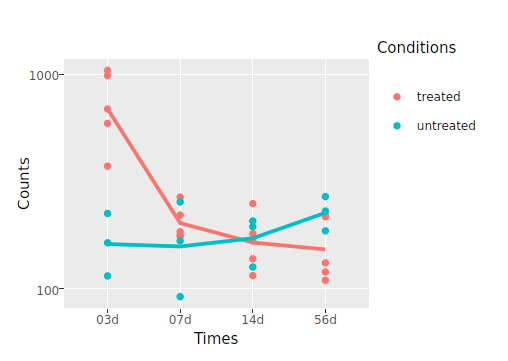
\includegraphics[width=10cm, keepaspectratio]{img/ticorser/gene_trend.png}
\caption[ticorser gene profile]{An example of interactive gene profile made with \gls{tic} package. Each dot represents the counts value of the gene in a sample. Colours identifies the conditions of the samples. The lines represent the gene trend over all time points.}
\label{fig:ticorsergenetrend}
\end{figure}


\subsubsection{keggmap}
Once detected \glspl{deg} it is really important to look for functional mechanisms regulated by up-regulated and down-regulated genes. 

\gls{tic} offers the possibility to plot \textit{keggmaps}\cite{Kanehisa2016} taking into account the $log_2(FC)$ of the genes involved in the graphical representation, through all the timepoints.
Indeed, using the \lstinline!plotKeggmap! function it enables to plot a \textit{keggmap}, using as input the counts and the design matrix, computing the $log_2(FC)$ at each time point, and showing it in the gene box inside the kegg map.

\begin{figure}[H]
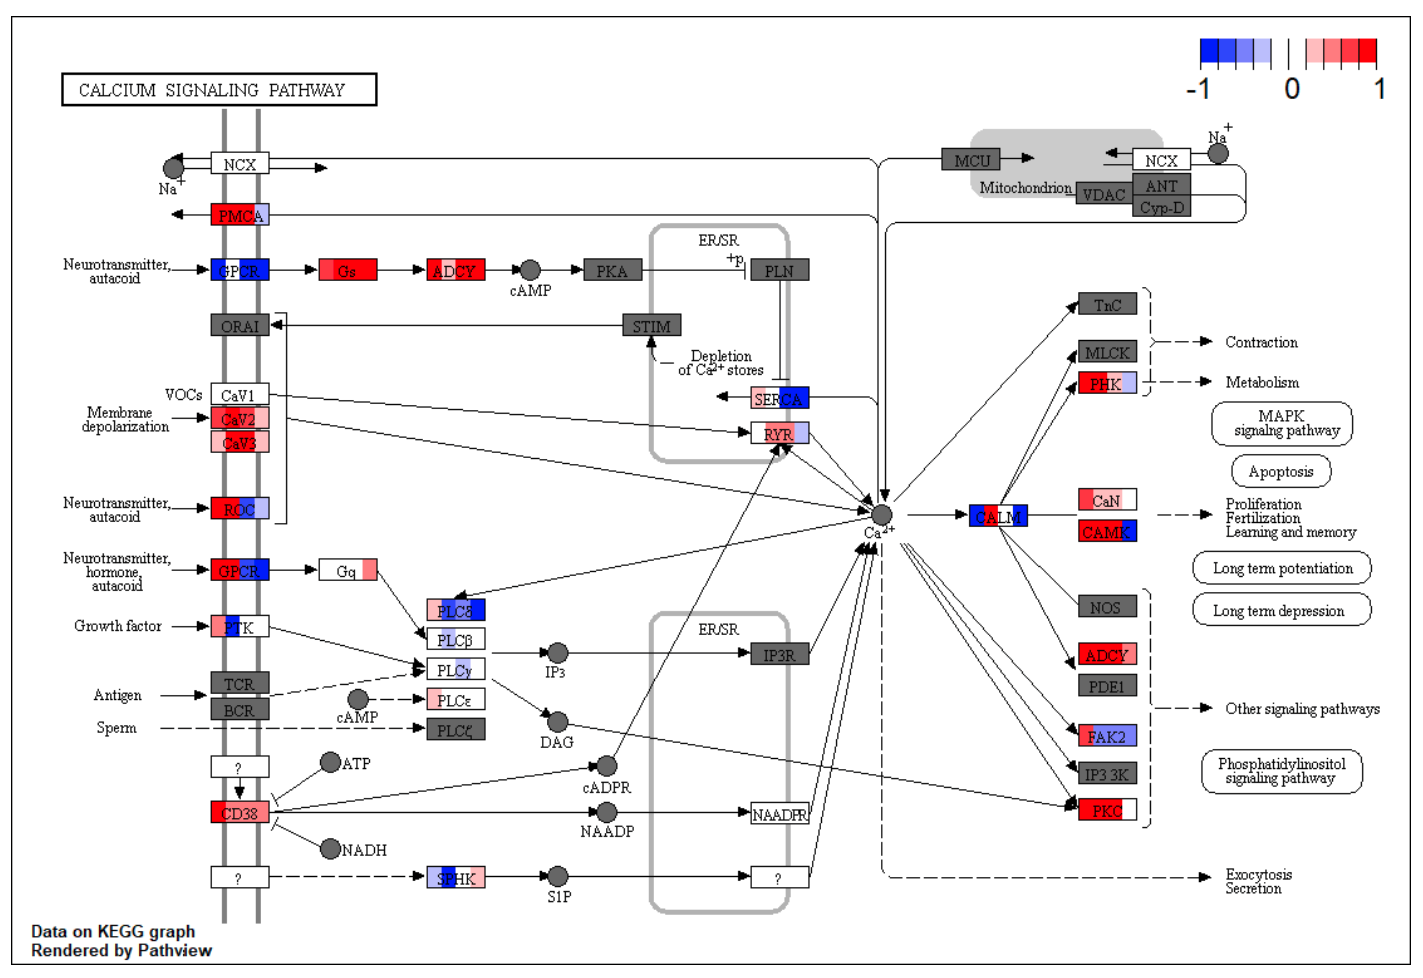
\includegraphics[width=12cm, keepaspectratio]{img/ticorser/keggmap_example.png}
\caption[ticorser keggmap]{add description}
\label{fig:ticorserkeggmap}
\centering
\end{figure}








